\documentclass[11pt,a4j]{article}
\usepackage[dvipdfmx]{graphicx,color}
\usepackage{wrapfig}
\setlength{\topmargin}{-1.5cm}
\setlength{\textwidth}{15.5cm}
\setlength{\textheight}{25.2cm}
\newlength{\minitwocolumn}
\setlength{\minitwocolumn}{0.5\textwidth}
\addtolength{\minitwocolumn}{-\columnsep}
%\addtolength{\baselineskip}{-0.1\baselineskip}
%
\def\Mmaru#1{{\ooalign{\hfil#1\/\hfil\crcr
\raise.167ex\hbox{\mathhexbox 20D}}}}
%
\begin{document}
\newcommand{\fat}[1]{\mbox{\boldmath $#1$}}
\newcommand{\D}{\partial}
\newcommand{\w}{\omega}
\newcommand{\ga}{\alpha}
\newcommand{\gb}{\beta}
\newcommand{\gx}{\xi}
\newcommand{\gz}{\zeta}
\newcommand{\vhat}[1]{\hat{\fat{#1}}}
\newcommand{\spc}{\vspace{0.7\baselineskip}}
\newcommand{\halfspc}{\vspace{0.3\baselineskip}}
\bibliographystyle{unsrt}
%\pagestyle{empty}
\newcommand{\twofig}[2]
 {
   \begin{figure}[h]
     \begin{minipage}[t]{\minitwocolumn}
         \begin{center}   #1
         \end{center}
     \end{minipage}
         \hspace{\columnsep}
     \begin{minipage}[t]{\minitwocolumn}
         \begin{center} #2
         \end{center}
     \end{minipage}
   \end{figure}
 }
%%%%%%%%%%%%%%%%%%%%%%%%%%%%%%%%%
%\vspace*{\baselineskip}
\begin{center}
{\LARGE \bf Synthetic Aperture Focusing Algorithm \\ for Ultrasonic Imaging}
\end{center}
\vspace{10mm}
%%%%%%%%%%%%%%%%%%%%%%%%%%%%%%%%%%%%%%%%%%%%%%%%%%%%%%%%%%%%%%%%
\section{Imaging Problem}
\hspace{\parindent}
In this article, we present our ultrasonic imaging method 
for a reasonably general model of a ultrasonic testing (UT) 
of a flawed plate as schematically shown in Fig.*. 
In this model, it is assumed that the incident ultrasonic wave is 
excited at a point $\fat{x}_s$ on the top plate surface.
The echoes returning from the flaw are also observed on the top surface 
over an aperture $\cal R$.
The ultrasonic echo signal captured with an transducer is usually given as a temporal 
 waveform, and is called an A-scan in the context of ultrasonic nondestructive testing.
We adopt this terminology in this article, and denote the A-scan captured 
at $\fat{x}$ as $a(\fat{x},t;\fat{x}_s)$ where $t$ is the time elapsed from 
the time of incident wave excitation. 
Since A-scans are captured on $\cal R$, the whole dataset 
 available for the imaging is written as 
\begin{equation}
	{\cal D} = \left\{
		a(\fat{x},t;\fat{x}_s)\left| \fat{x}\in {\cal R},t>0 \right.
	\right\}.
	\label{eqn:bscan_data}
\end{equation}
For given dataset $\cal D$, we consider synthesizing an image $I(\fat{x}_P)$ 
of the unknown flaw, thereby estimate the location and size of the flaw.
%%%%%%%%%%%%%%%%%%%%%%%%%
\section{Synthetic Aperture Imaging Algorithm}
\hspace{\parindent}
The present synthetic imaging algorithm may be divided into two parts.
The first part is a delay-and-sum operation on the measured A-scans ${\cal D}$. 
The second part is a sampling or projection operation on the resulting summed A-scan.
The delay law and the nature of the samplig/projection are both related closely 
to the travel time of the ultrasonic wave.
It is thus convenient to introduce a handy notation for the travel time. 
When an ultrasonic wave travels from $\fat{y}$ to $\fat{x}$ 
 taking a flight time $t_f$, we write
\begin{equation}
	t_f=T_f(\fat{x},\fat{y}).
	\label{eqn:Tf}
\end{equation}
It reads "the travel time from \fat{y} to \fat{x} is $t_f$".
In eq.(\ref{eqn:Tf}), it is meant that $t_f$ is a single travel time, while 
$T_f$ is the function which returns the travel time for given point of 
departure and arrival. 
To process an A-scan with the help of time-of-flight concept, it is necessary to 
decompose $a(\fat{x},t;\fat{x}_s)$ into the incident and scattered components as 
\begin{equation}
	a(\fat{x},t;\fat{x}_s)=
	a^{in}(\fat{x},t;\fat{x}_s)
	+
	a^{sc}(\fat{x},t;\fat{x}_s).
	\label{eqn:wv_split}
\end{equation}
As in eq.(\ref{eqn:wv_split}), quantities associated with the incident and scattered wave 
components are and will be denoted with the superscripts "{\it in}" and "{\it sc}", respectively.
With this decomposition, we may associate a flight time
\begin{equation}
	t^{in}(\fat{x})=T_f(\fat{x},\fat{x}_s), (\fat{x} \in {\cal R})
	\label{eqn:def_tin}
\end{equation}
with the incident wave component $a^{in}(\fat{x},t;\fat{x}_s)$. 
If $t^{in}(\fat{x})$ is estimated for every $\fat{x} \in {\cal R}$, 
the incident wave pulse in each A-scan can be aligned at the origin 
of the coordinate $t=0$ by translating $a(x,t)$ by $t^{in}(\fat{x})$ as 
$a\left(\fat{x},t+t^{in}(\fat{x})\right)$.
The A-scans translated thus are then superimposed as 
\begin{equation}
	\bar{a}^{in}(t)=\int_{\cal R} a\left(\fat{x},t+t^{in}(\fat{x})\right)dx,
	\label{eqn:asum_in}
\end{equation}
so that the incident wave pulse in $\bar{a}^{in}(t)$ be amplified to a degree 
dependent on the accuracy of the estimated travel time.
Clearly, eq.(\ref{eqn:asum_in}) is a delay-and-sum in which the waveform $a(\fat{x},t)$ 
is delayed by $-t^{in}(\fat{x})$ and summed over the aperture $\cal R$.

A summed A-scan similar to eq.(\ref{eqn:asum_in}) may be obtained for the 
scattered wave component $a^{sc}(\fat{x},t)$. 
Associating the flight time, however, with the scattered wave component is not straightforward. 
This is because scattered waves are generated at every point on the scattering object. 
Consequently, it is not possible to pinpoint where exactly is a scattered wave is originated from. 
 A simple and practical trick to circumvent this difficulty is to model the scattering object 
 as a collection of small, point-like scatterers distributed densely but discretely over 
 the surface of the object. Then the flight time can be assigned to each constituent point scatterer 
 with no ambiguity. This approach may be formulated more rigorously if we discretize an 
 integral representation of the scattered field, which is beyond the scope of this article.
When one of the point scatteres is located at $\fat{x}_P$, the flight time for the scattered wave 
 is given by 
\begin{equation}
	t_P^{sc}(\fat{x})=
	T_f(\fat{x}_P,\fat{x}_s)
	+
	T_f(\fat{x},\fat{x}_P).
	\label{eqn:tsc}
\end{equation}
The subscript $P$ in eq.(\ref{eqn:tsc}) is to remind that the flight time depend 
on the location of the point scatterer.
Then we can align and amplify the scattered wave packets at $t=0$ by the following delay-and-sum operation. 
\begin{equation}
	\bar{a}^{sc}_P(t)=\int _{\cal R} a^{sc}(\fat{x},t+t^{sc}_P(\fat{x}))d\fat{x}
	\label{eqn:asum_sc}
\end{equation}
Obviously, the degree of amplification depends on the accuracy of the estimation of $t^{sc}_P$. 
It is equally or more important to note that the amplification would not occur if there were not 
the scatterer at $\fat{x}_P$ in the first place, or if the scattered waves from $\fat{x}_P$ did 
not take the path that has been considered in estimating $t^{sc}_P(\fat{x})$.
This suggests that the summed A-scan $\bar a^{sc}_P$ can be used to assess the likelihood that 
a point scatterer is actually at $\fat{x}_P$. 
Although variety of different measures of likelihood can be invented, one of the 
most simplest methods is the use of sampling or projection. 
If we write the sampling/projection operation symbolically as ${\cal S}$, 
we can think of creating a likelihood map 
\begin{equation}
	%I(\fat{x}_P)={\cal S} \left\{ \bar{a}^{sc}_P(t) \right\}
	I(\fat{x}_P)={\cal S} \left[ \bar{a}^{sc}_P(t) \right], 
	(\fat{x}_P \in A),
	\label{eqn:image}
\end{equation}
over an area $A$, and is shown as an image of the scattering object.
To take this imaging approach, the operator $\cal S$ need to be specified. 
 The simplest choice for $\cal S$ is a sampling by Dirac's delta function 
\begin{equation}
	{\cal S} \left[ 
		\bar{a}^{sc}_P(t) 
		\right]
	=\left<
	\delta(t),\, \bar{a}^{sc}_P
	\right>
	=
	\bar{a}^{sc}_P(0)
\end{equation}
where $\left<\cdot,\, \cdot \right>$ is the dot product
\begin{equation}
	\left< f,g \right>=\int f(t)g(t) dt.
	\label{eqn:}
\end{equation}
of two well behave functions $f$ and $g$.
The intention is obvious because the $\bar{a}^{sc}_P$ is constructed so that the 
wave packet is amplified at $t=0$. However, this is not a good choice when the scattered 
wave packet is not an ideal pulse. In real A-scans, the peak amplitude of a  
wave packet always comes after the theoretically estimated flight time. 
The Dirac's delta sampling therefore results in an underestimation of the underlying wave packet. 
A better alternative is a projection using a reference signal. 
In this study, we adopts the following. 
\begin{equation}
	{\cal S} \left[ 
		\bar{a}^{sc}_P(t) 
		\right]
	=
	\frac{
		\left< 
			\bar{a}^{in}(t) 
			,\bar{a}^{sc}_P(t) 
		\right>
	}{
		\left\| 
			\bar{a}^{in}(t) 
		\right\|^2
	}
	\label{eqn:S_cor}
\end{equation}
where $\left\| f \right\|^2 =\left< f,f \right>$. 
In eq.(\ref{eqn:S_cor}), an unknown delay is automatically compensated by the 
delay in the reference signal.  
We can further generalize the projection approach e.g. to 
\begin{equation}
	{\cal S} \left[ 
		\bar{a}^{sc}_P(t) 
		\right]
	=
	\left\|a^{in}(t)*a^{sc}(t)\right\|_p
	\label{eqn:}
\end{equation}
where $p$ is a non-negative integer, $*$ denotes a convolution product, 
and $\left\| f  \right\|_p= \left\{\int \left| f\right|^p\right\}^{\frac{1}{p}}$ 
is the usual $p-$norm. However, we're not going to elaborate the projection operator. 
Rather, we adopt a relatively simple projection operator (\ref{eqn:S_cor}) and 
 investigate how it works with measured waveforms in an attempt of 
 imaging by eq.(\ref{eqn:image}) with eqs.(\ref{eqn:asum_in}) and (\ref{eqn:asum_sc}).
\section{Numerical Implementation}
\subsection{Incident and scattered wave splitting}
Let $u(x,t)$ be an wave amplitude at position $x$ and time $t$, and let 
$U(k,\omega)$ be the Fourier transform of $u(x,t)$ given by 
\begin{equation}
	U(k,\omega)=\frac{1}{\left(2\pi\right)^2}
	\int\int u(x,t)e^{-ikx+i\omega t} dxdt.
	\label{eqn:}
\end{equation}
Then, the spectral representation of the wave field $u(x,t)$ may be written as 
\begin{equation}
	u(x,t)=\int U(k,\omega) e^{i(kx-\omega t)} dkd\omega.
	\label{eqn:U2u}
\end{equation}
Noting that the exponential function $e^{ikx-i\omega t}$ represents a wave 
traveling in $x>0(<0)$ direction when $k\omega >0(<0)$, 
the wave field $u(x,t)$ can be split into the components traveling in the 
positive and negative $x$ directions by a filtered Fourier transform:
\begin{equation}
	u^{\pm}(x,t)=\int U(k,\omega)H(\pm k\omega) e^{i(kx-\omega t)} dkd\omega
	\label{eqn:kw_filter}
\end{equation}
where $H(s)$ is the Heaviside unit step function.
\begin{equation}
	H(s)=\left\{
	\begin{array}{cc}
		1 & (s >0) \\
		0 & (s <0)
	\end{array}
	\right. .
	\label{eqn:}
\end{equation}
In our imaging algorithm, the splitting of eq.(\ref{eqn:wv_split}) is found 
by the filtered Fourier transform (\ref{eqn:U2u}), considering that the wave traveling 
toward and away from the flaw as the incident and the scattered wave component,respectively.
%%%%%%%%%%%%%%%%%5
\subsection{Construction of the travel time function}
\hspace{\parindent}
For a given set of source and observation points in a plate, 
there are infinitely many possible wave propagation paths 
due to reverberation.
To implement the imaging algorithm, we have to identify a path that 
is most likely to be taken by the incident/scattered wave. 
The travel time can evaluated for the selected path first by 
measuring the path length and then dividing the length by the 
wave velocity $c$.
If the wave mode conversion is considered, the number of possible 
propagation paths to be considered increases exponentially as the 
number of reflection becomes larger. This would make the travel time 
analysis computationally too demanding. In this study, therefore, 
we look exclusively at the mode preserving paths, on which the wave 
mode does not change before and after the reflection.
%no the path does not split upon the reflection. 
According to the Snell's law, the angles of incident and reflection are 
identical with if the wave mode is not changed.
This make the travel time analysis extremely simple, and consequently 
the travel time function for any propagation path can be written explicitly. 


There are four types of travel paths for the waves reverberate in a plate 
as depicted in Fig.\ref{eqn:fig1}. Due to the mode preservation assumption, 
a propagation path of any type can be straighten up. Thus, the path length can 
be obtained by a straight forward application of Pythagoras theorem. 
To formulate this procedure, let $a$ and $b$ be the heights of the source 
and the observation points, respectively, measured from the bottom of 
the plate of thickness $h$. Similarly, let $a'$ and $b'$ be the depths 
of the source and the observation points from the top surface, respectively. 
If we take type 1 path, for example, the straightened path may be drawn 
as shown in Fig.\ref{eqn:fig2} for $n=3$ where $n$ is the number of reflection.
It is easy to verify that the path length $L$ is given as
\begin{equation}
	L=\sqrt{X^2+H^2}, \ \ H=a+b+(n-1)h
	\label{eqn:L3}
\end{equation}
where $X$ is the horizontal distance between the source and the observation points.
The formulae for the remaining three types of path may be obtained in a similar fashion.
Furthermore, the resulting formulae for all of the four path types are put together 
if we introduce a variable $\sigma$ to denote the wave direction as 
\begin{equation}
	\sigma=
	\left\{
	\begin{array}{cc}
		0 & {\rm for \: initially\: down-going\: wave} \\
		1 & {\rm for \: initially\: up-going\: wave} 
	\end{array}
	\right.
	,
	\label{eqn:def_sigma}
\end{equation}
and a variable subsidiary to $n$ as 
\begin{equation}
	n'=n \: {\rm mod} 2.
	\label{eqn:}
\end{equation}
Then the height $H$ of the straightened path may be written as 
\begin{equation}
	H(\sigma,\, n) = h_0+h_n+(n-1)h
	\label{eqn:}
\end{equation}
with 
\begin{equation}
	h_0=
	\left\{
	\begin{array}{cc}
		a &  (\sigma=0)\\
		a'&  (\sigma=1)
	\end{array}
	\right.
	, \ \ 
	h_n=
	\left\{
	\begin{array}{cc}
		b &  (\sigma \neq n')\\
		b'&  (\sigma = n')
	\end{array}
	\right.
	.
	\label{eqn:}
\end{equation}
Finally, the path length $L$ and the travel time $T_f$ are 
 given respectively as follows.
\begin{equation}
	L(\sigma ,n)=\sqrt{X^2+ H^2(\sigma ,n)}, \ \ 
	T_f(\fat{x},\fat{y};\sigma,n)=\frac{L(\sigma,n)}{c}
	\label{eqn:}
\end{equation}
where $c$ has been assumed to be constant.
%--------------------
\begin{figure}[h]
	\begin{center}
	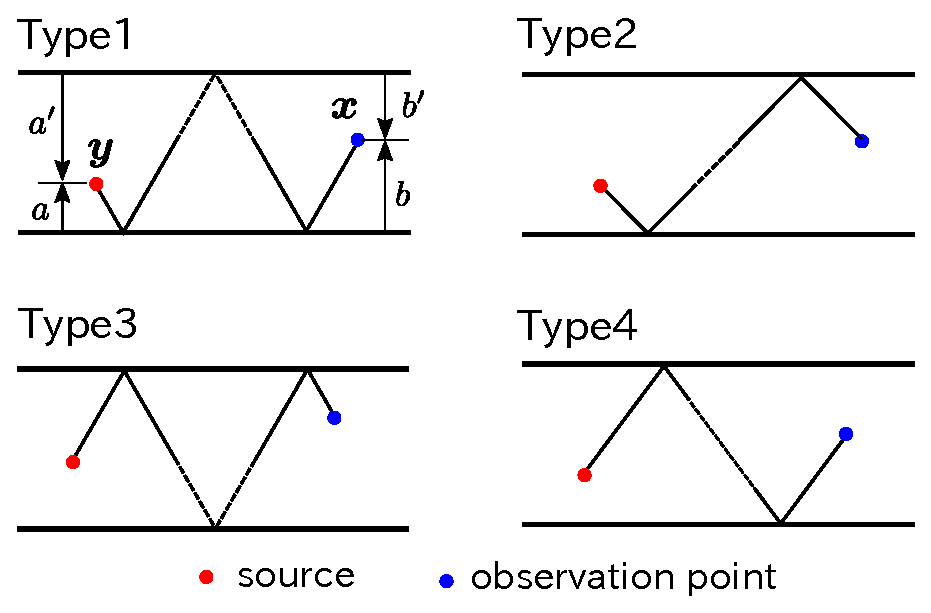
\includegraphics[width=0.7\linewidth]{paths.eps} 
	\end{center}
	\caption{
		Types of paths for the mode preserving wave propagation. 
	} 
	\label{fig:fig1}
\end{figure}
%--------------------
\begin{figure}[h]
	\begin{center}
	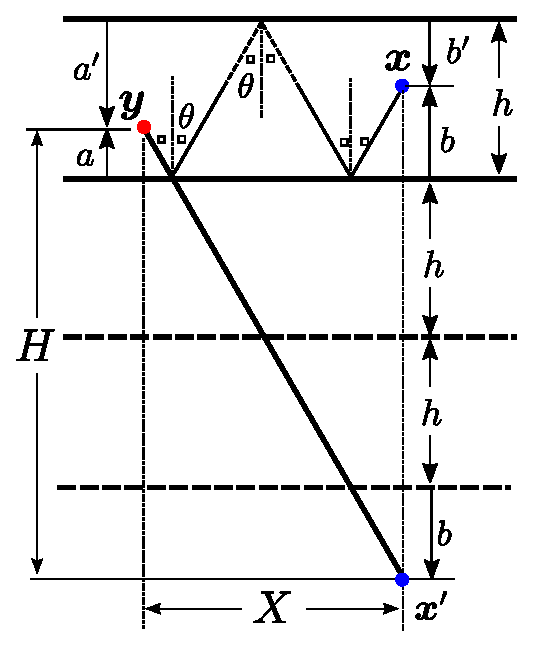
\includegraphics[width=0.5\linewidth]{length.eps} 
	\end{center}
	\caption{
		A straightened propagation paths, and the heigt $H$ and the 
		horizontal distance $L$.
	} 
	\label{fig:fig2}
\end{figure}
%--------------------
%--------------------
\end{document}

